\documentclass[a4paper]{article}
\usepackage{graphicx}
\usepackage{amsmath}
\usepackage[bookmarks = true, colorlinks=true, linkcolor = black, citecolor = black, menucolor = black, urlcolor = black]{hyperref}
\usepackage[spanish,activeacute]{babel}
\usepackage{lmodern}
\usepackage{listings}
\usepackage{adjustbox}
\usepackage{float}
\renewcommand{\baselinestretch}{1} % Interlineado. 1 es estandar
\usepackage[utf8x]{inputenc}
\usepackage[T1]{fontenc}
\usepackage[square,sort,comma,numbers]{natbib}
\usepackage{mathtools}
\usepackage{fancyhdr}
\fancyhead[R]{2020}\fancyhead[L]{UNC - FCEFyN} \fancyfoot[C]{\thepage}
\pagestyle{fancy}
\usepackage[numbered]{bookmark} % Para que figure las secciones en el PDF

\begin{document}
\begin{titlepage}
	
	{\scshape\LARGE Universidad Nacional de Córdoba \par}
	%\vspace{1cm}
	{\Large Facultad de Ciencias Exactas, Físicas y Naturales \par}
	\vspace{0.5cm}
	\centering
	
\includegraphics[width=0.5\textwidth]{unc.png}
	\par\vspace{0.5cm}
	\vspace{0.5cm}
	{\scshape\Large TRABAJO PRÁCTICO N°2\par}
	{\large Sistemas Operativos II\par}
	\vspace{1.5cm}
	{\large\bfseries OpenMP \par}
	\vspace{1.5cm}
	{\Large\bfseries Gerardo Collante\par}
	\vfill
	Profesor\par
	Ing.~Agustín \textsc{Martina}

	\vfill

% Bottom of the page
	{\large \today\par}
\end{titlepage}

%This document is an example of \texttt{natbib} package using in bibliography
%management. Three items are cited: \textit{The \LaTeX\ Companion} book 
%\cite{latexcompanion}, the Einstein journal paper \citep{einstein}, and the 
%Donald Knuth's website. The \LaTeX\ related items are 
%\citet{poole1998}. 

\tableofcontents

\clearpage

\section{Introducción}
\subsection{Propósito}
Los niveles de integración electrónica han permitido la generación de procesadores de arquitecturas \textit{multiprocess}, \textit{multicore} y ahora \textit{many integrated core (MIC)}. Este avance hace necesario que los programadores cuenten con un profundo conocimiento del hardware sobre el que se ejecutan sus programas, y que dichos programas ya no pueden ser monoproceso.
Entre las técnicas y estándares más utilizados para sistemas de memoria compartida y memoria distribuida, se encuentra OpenMP y MPI respectivamente.

\subsection{Objetivo}

El objetivo del presente trabajo práctico es que el estudiante sea capaz diseñar una solución que utilice el paradigma de memoria distribuida, utilizando OpenMP.

\section{Descripción}

\subsection{Requerimientos}
Para realizar el presente trabajo práctico es necesario instalar las librerías NetCDF4 en el sistema sobre el cual se diseñe, desarrolle y testee la solución al problema.
Estas librerías permiten compartir información tecnológica y científica en un formato auto-definido, independiente de la arquitectura del sistema. Por ello se transformó en un estándar abierto.
La librería tiene versiones para diferentes lenguajes pero se utilizará la de \textit{C}.
Como \textit{e.g.} del uso de este formato de datos se tiene la red de radares meteorológicos \textit{NexRad} y la constelación de satélites GOES, ambos disponibles públicamente. 

\subsection{Problema a desarrollar}

El satélite GOES16, utilizando su canal 2, obtuvo la información almacenada en un archivo con extensión \textit{.nc}.
El nombre del archivo nos informa del instrumento utilizado (ABI-L2-CMIPF-M6C02), el canal (C02), el satelite que lo creo (G16), el $timestamp$ de la creación del archivo, y por último del inicio y final del barrido. 
El canal 2, correponde a la longitud de onda de $0.64 \mu m$, correspondiente al espectro de la luz visible y posee una resolución de $500m$, $i.e.$ cada pixel de la imagen corresponde a 500 metros de la superficie aproximadamente. A continuación se muestra una imagen de la salida de este archivo en la Fig.\ref{fig:imgsatelital}.

\begin{figure}[H]
	\begin{center}		
	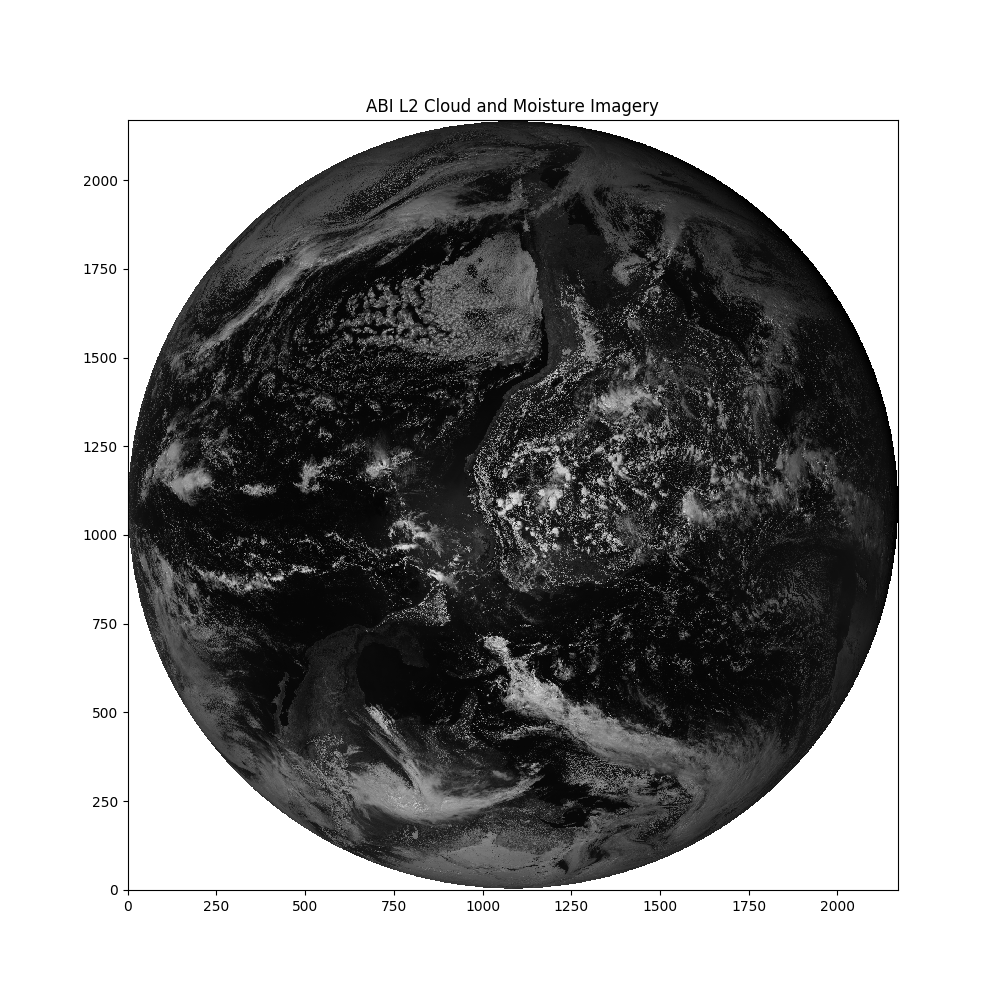
\includegraphics[width=0.75\textwidth]{../imagenOriginal.png}
  	\caption{Imagen original obtenida del satélite.}
  	\label{fig:imgsatelital}
  	\end{center}
\end{figure}

Dentro del archivo hay una variable llamada CMI, de una matriz cuadrada de \texttt{float} de 21696 filas por columnas, con la que se generó la imagen anterior. Cada punto de la matriz, corresponde a un pixel de la imagen y posee el valor del "brillo" en ese punto. Fuera del planeta, todos los valores son $nan$.

Se pide que, se implemente un algoritmo que aplique un filtro de borde sobre toda la matriz de la imagen del planeta. La imagen filtrada se obtiene a partir de la siguiente convolución:

\begin{equation}
	g(y,z) = w*f(x,y)=\sum_{s=-a}^{a}  \sum_{t=-b}^{b}  w(s,t) f(x-s, y-t)
\end{equation}

Donde $g(x,y)$ es la imagen filtrada, $f(x,y)$ es la imagen original y $w$ es la matriz que se define a continuación, con limites $-a \leq s \leq a$ y $-b \leq t \leq b$.

\begin{center}

$
\omega=
  \begin{bmatrix}
    -1 & -1 & -1\\
    -1 & 8 & -1\\
    -1 & -1 & -1\\
    
  \end{bmatrix}
$

\end{center}

\clearpage

\section{Desarrollo}
\subsection{Metodología de trabajo}
Se podría definir en los siguientes pasos:
\begin{itemize}
\item Se optó en principio por desarrollar una solución de manera secuencial en C.
\item Una vez lista esta solución se empiezan a agregar las directivas de OpenMP para paralelizar y así aprovechar el uso de los $threads$ del procesador.
\item Una vez completado esta fase se procede a correr el programa en el cluster de la facultad, realizando y documentando las pruebas para posteriormente estos resultados ser analizados.
\end{itemize}

\subsection{Descripción del algoritmo}
Se convierte el archivo .nc en una matriz de \texttt{short} de 21696x21696, que luego se procede a convolucionar con el $kernel$ a través de un cuádruple $for$ anidado y esta es guardada en otra matriz. 

Es importante allocar el tamaño de estas matrices ya que son muy grandes y no hacerlo podría provocar errores de $segmentation fault$.
Luego se procede a crear otro archivo $.nc$, y se sustituyen los valores de la matriz original. Para obtener la imagen se utiliza un ejecutable $Python$, que se muestra a continuación en la Fig  \ref{fig:imgfiltrada}.

\begin{figure}[H]
	\begin{center}		
	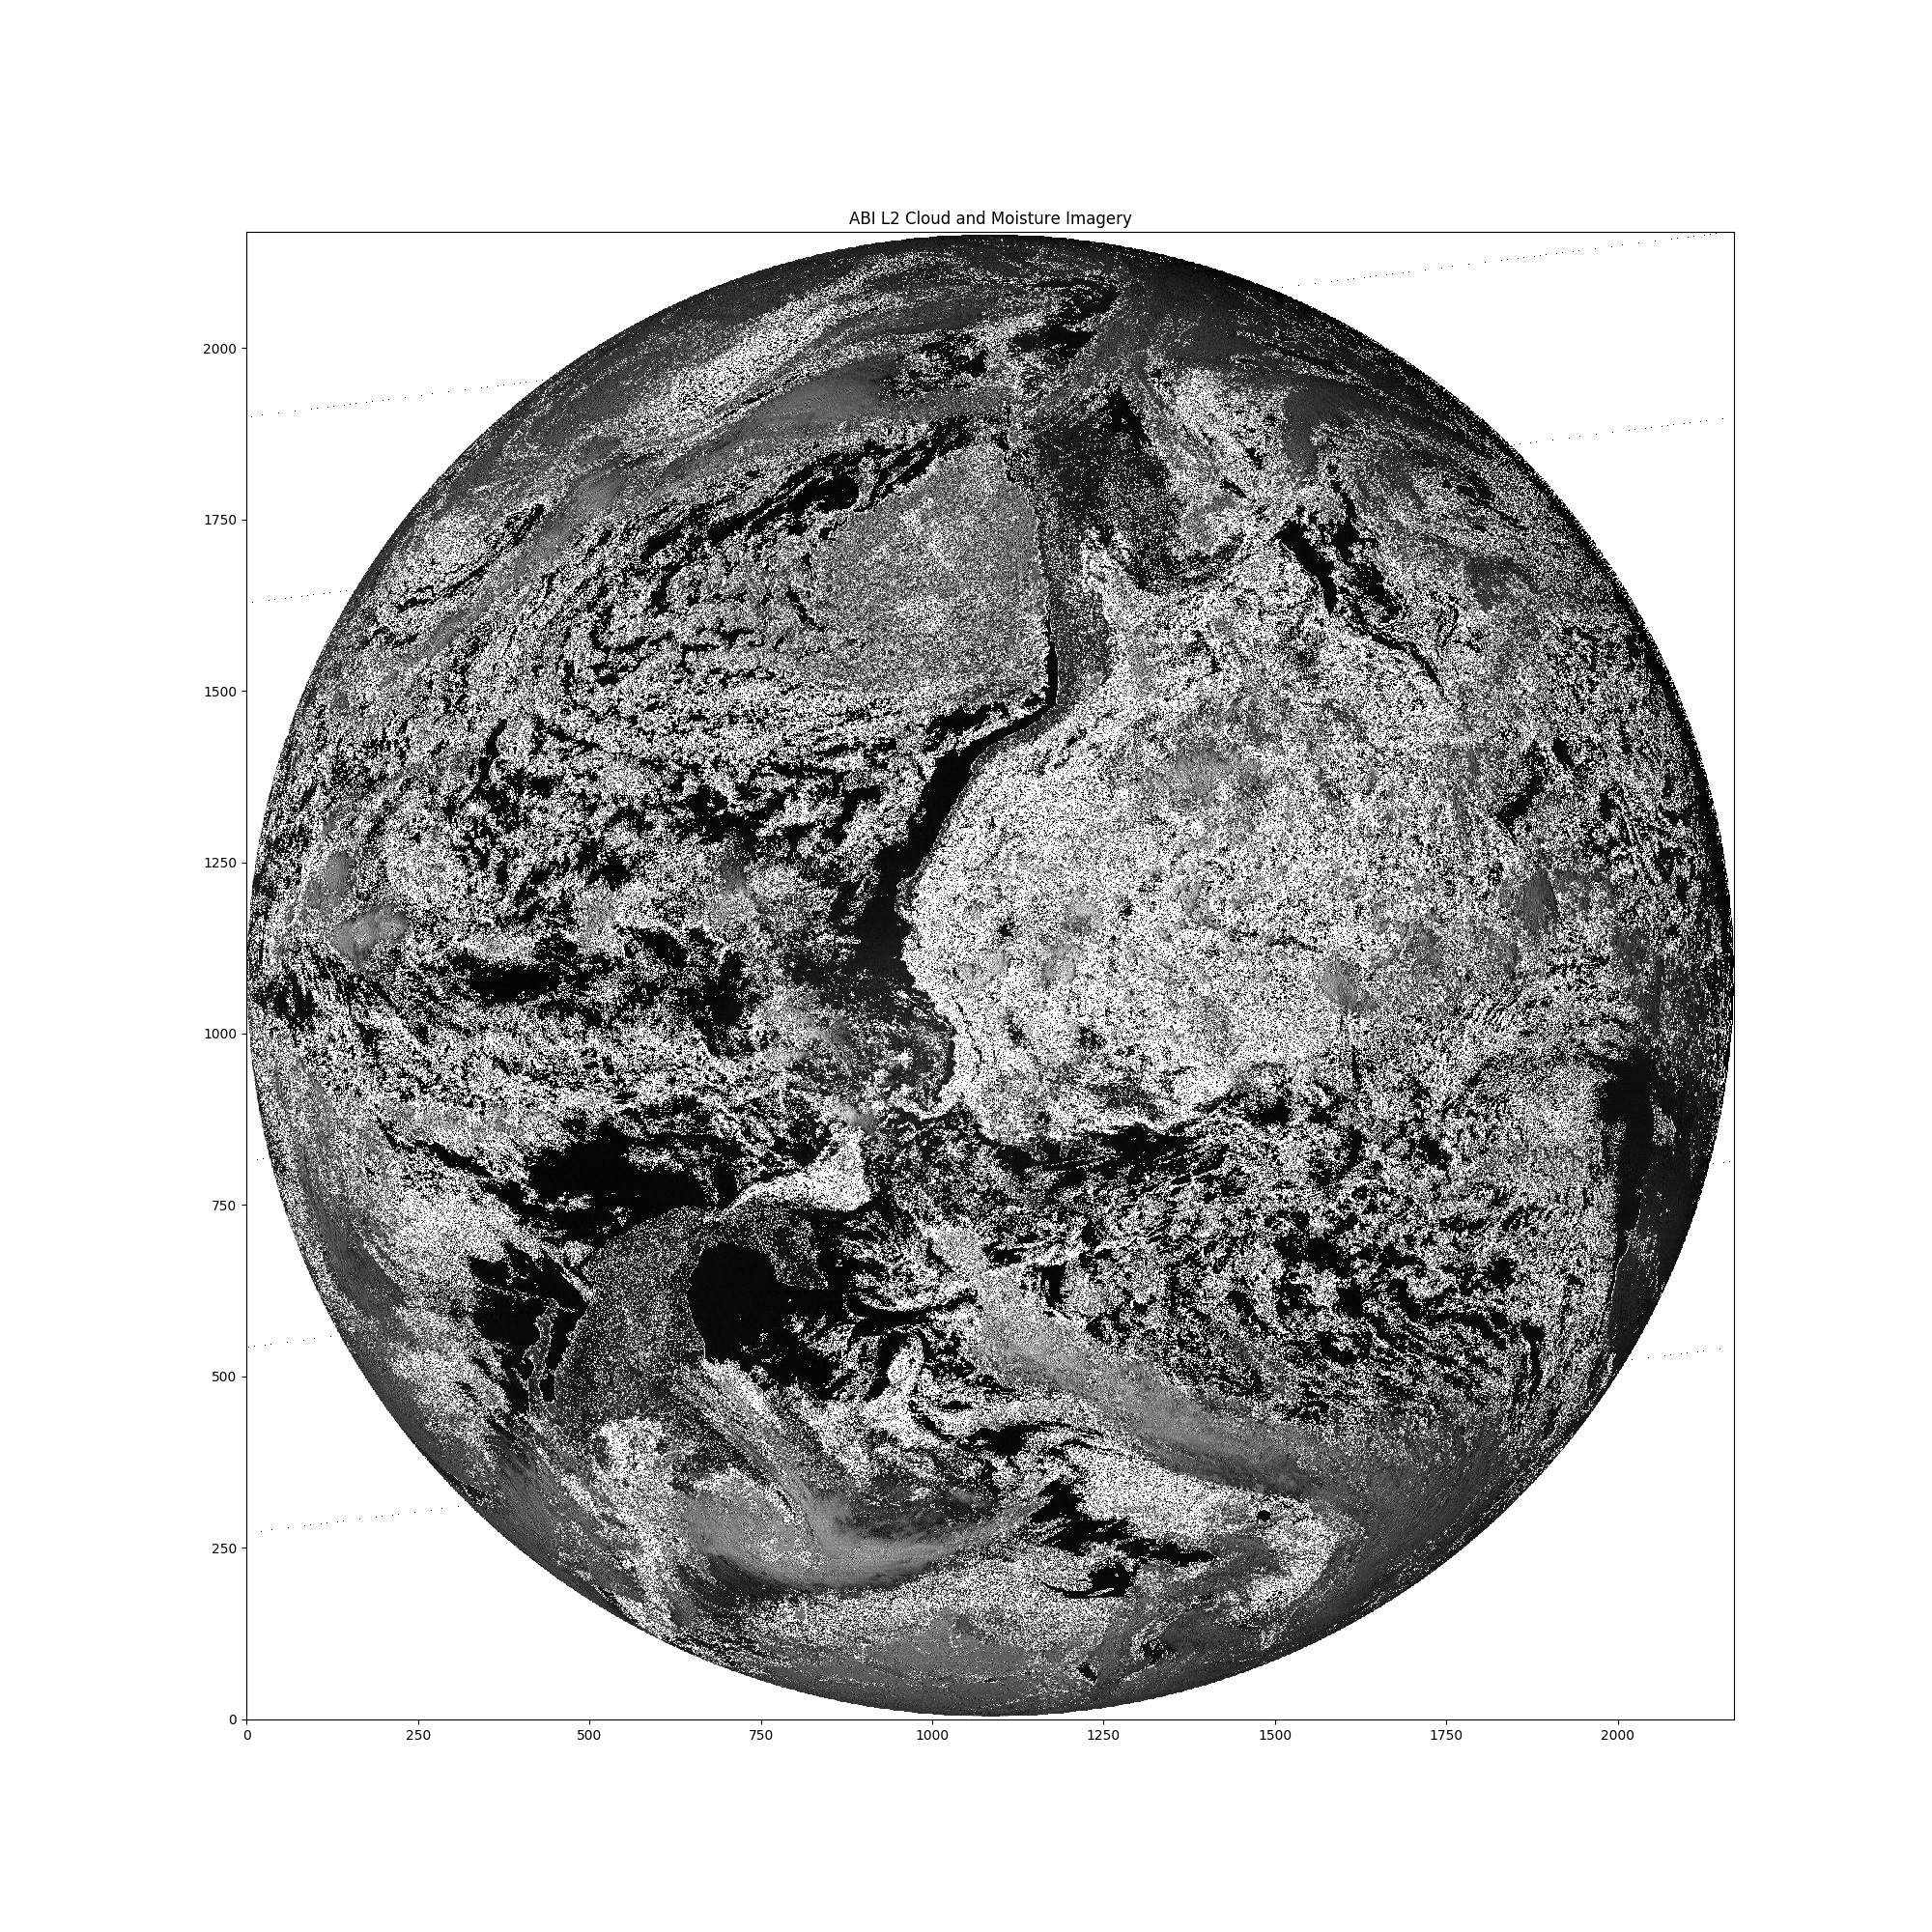
\includegraphics[width=0.75\textwidth]{../imagenFiltrada.png}
  	\caption{Imagen filtrada luego del procesamiento.}
  	\label{fig:imgfiltrada}
  	\end{center}
\end{figure}


\subsection{Pruebas}
\subsubsection{Host local}
Las pruebas fueron realizadas en un host local con las siguientes características técnicas:
\begin{itemize}
\item Procesador Intel® Core™ i3-4100M CPU @ 2.5GHz de 4 hilos físicos y 8 lógicos.
\item 4GB RAM.
\end{itemize}
Se corrió el programa con 1, 2, 4, 8 hilos con 30 pasadas cada uno para obtener un promedio, obteniéndose los resultados observados en el Cuadro \ref{tab:tablanotebook} y Cuadro \ref{tab:tabpromnote}.

\begin{figure}[H]
	\begin{center}		
	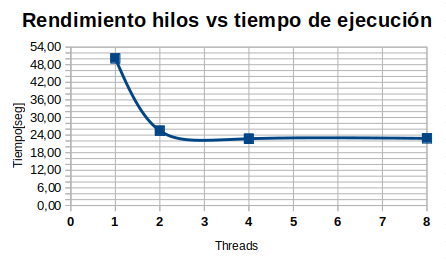
\includegraphics[width=0.6\textwidth]{002.png}
  	\caption{Gráfico comparativo host local.}
  	\label{fig:grafnote}
  	\end{center}
\end{figure}

\begin{table}[]
\centering
\begin{tabular}{lllll}
         & \multicolumn{4}{c}{\textbf{CANTIDAD DE HILOS}}                                                \\ \hline
Pasada   & \multicolumn{1}{c}{1} & \multicolumn{1}{c}{2} & \multicolumn{1}{c}{4} & \multicolumn{1}{c}{8} \\
1       & 51,95 & 27,15 & 23,50 & 23,06 \\
2       & 50,53 & 26,26 & 23,02 & 22,91 \\
3       & 50,32 & 26,10 & 22,77 & 22,90 \\
4       & 50,19 & 26,00 & 22,76 & 22,90 \\
5       & 50,16 & 25,73 & 22,74 & 22,89 \\
6       & 50,15 & 25,43 & 22,74 & 22,88 \\
7       & 50,11 & 25,42 & 22,74 & 22,88 \\
8       & 50,10 & 25,41 & 22,73 & 22,88 \\
9       & 50,09 & 25,37 & 22,73 & 22,88 \\
10      & 50,05 & 25,37 & 22,72 & 22,88 \\
11      & 50,05 & 25,34 & 22,71 & 22,88 \\
12      & 50,05 & 25,33 & 22,71 & 22,87 \\
13      & 50,04 & 25,33 & 22,71 & 22,87 \\
14      & 50,04 & 25,33 & 22,71 & 22,87 \\
15      & 50,04 & 25,32 & 22,71 & 22,87 \\
16      & 50,04 & 25,32 & 22,70 & 22,86 \\
17      & 50,04 & 25,31 & 22,70 & 22,86 \\
18      & 50,04 & 25,31 & 22,70 & 22,86 \\
19      & 50,03 & 25,31 & 22,70 & 22,86 \\
20      & 50,03 & 25,31 & 22,70 & 22,86 \\
21      & 50,03 & 25,31 & 22,70 & 22,86 \\
22      & 50,03 & 25,31 & 22,70 & 22,86 \\
23      & 50,03 & 25,31 & 22,70 & 22,85 \\
24      & 50,03 & 25,30 & 22,70 & 22,85 \\
25      & 50,03 & 25,30 & 22,70 & 22,85 \\
26      & 50,03 & 25,30 & 22,70 & 22,85 \\
27      & 50,03 & 25,30 & 22,70 & 22,85 \\
28      & 50,01 & 25,30 & 22,69 & 22,85 \\
29      & 49,87 & 25,30 & 22,67 & 22,85 \\
30      & 49,80 & 25,30 & 22,66 & 22,84 \\ \hline
PROMEDIO & 50,13                 & 25,48                 & 22,75                 & 22,87                 \\
DESVEST & 0,36  & 0,40  & 0,15  & 0,04  \\ \hline
\end{tabular}
\caption{Tabla de resultados host local.}
\label{tab:tablanotebook}
\end{table}

\begin{table}[]
\centering
\begin{tabular}{lllll}
\textbf{HILOS} & \textbf{PROMEDIO} & \textbf{DESVEST} & \textbf{MAX}   & \textbf{MIN}   \\ \hline
1     & 50,13    & 0,36    & 50,50 & 49,77 \\
2     & 25,48    & 0,40    & 25,89 & 25,08 \\
4     & 22,75    & 0,15    & 22,90 & 22,59 \\
8     & 22,87    & 0,04    & 22,91 & 22,84
\end{tabular}
\caption{Promedios host local.}
\label{tab:tabpromnote}
\end{table}

Las pruebas demostraron que a partir de 2 núcleos la velocidad de ejecución disminuía a la mitad, pero a medidas que se iban agregando núcleos la diferencia no era demasiada.

\subsubsection{Cluster}
Las pruebas se realizaron en el cluster de la Universidad Nacional de Córdoba que cuenta con las siguientes características:
\begin{itemize}
\item Procesador Intel® Xeon™ Gold 6130 CPU @ 2.10GHz de 32 hilos físicos y 64 lógicos.
\item 64GB RAM.
\end{itemize}
Se corrió el programa con 1, 2, 4, 8, 16, 32, 64 y 128 hilos con 30 pasadas cada uno para obtener un promedio, obteniéndose los resultados del Cuadro \ref{tab:tablecluster} y Cuadro \ref{tab:promcluster}.


\begin{figure}[H]
	\begin{center}		
	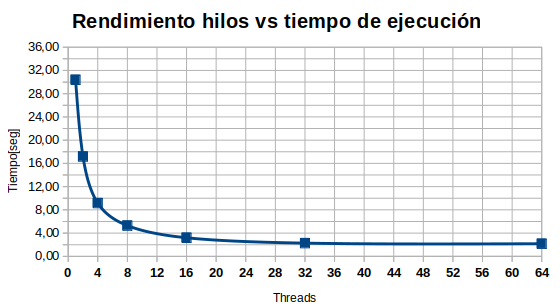
\includegraphics[width=0.6\textwidth]{003.png}
  	\caption{Gráfico comparativo cluster.}
  	\label{fig:grafcluster}
  	\end{center}
\end{figure}

Se observa que se obtiene una relación cuadrática inversa entre la cantidad de núcleos utilizados y el tiempo de ejecución del algoritmo, obteniendo una relación entre las variables.

También se concluye que a medida que se acerca al límite de hilos físicos no aporta ningún beneficio utilizar más que los que posee el host, ya que se solapan y se pierde tiempo de procesador realizando cambios de contexto entre estos.


\begin{table}[H]
\centering
\begin{tabular}{lcccc}
\textbf{HILOS} & \textbf{PROMEDIO} & \textbf{DESVEST} & \textbf{MAX} & \textbf{MIN} \\ \hline
1              & 30,39             & 0,65             & 31,04        & 29,74        \\
2              & 17,18             & 0,54             & 17,72        & 16,64        \\
4              & 9,17              & 0,34             & 9,51         & 8,82         \\
8              & 5,30              & 0,15             & 5,45         & 5,15         \\
16             & 3,20              & 0,10             & 3,30         & 3,10         \\
32             & 2,27              & 0,12             & 2,40         & 2,15         \\
64             & 2,17              & 0,07             & 2,24         & 2,10         \\
128            & 2,57              & 0,21             & 2,77         & 2,36        
\end{tabular}
\caption{Promedios cluster.}
\label{tab:promcluster}
\end{table}


\begin{table}[H]
\centering
\begin{tabular}{lcccccccc}
         & \multicolumn{8}{c}{\textbf{CANTIDAD DE HILOS}}                    \\ \hline
Pasada   & 1     & 2     & 4     & 8    & 16   & 32   & 64   & 128  \\
1        & 30,46 & 17,02 & 9,19  & 5,11 & 3,03 & 2,21 & 2,38 & 2,58 \\
2        & 31,69 & 16,92 & 8,66  & 5,23 & 3,19 & 2,29 & 2,14 & 2,35 \\
3        & 30,50 & 17,58 & 9,23  & 5,13 & 3,22 & 2,39 & 2,06 & 2,11 \\
4        & 30,40 & 17,16 & 9,20  & 5,06 & 3,22 & 2,31 & 2,06 & 2,08 \\
5        & 31,17 & 16,77 & 8,81  & 5,26 & 3,34 & 2,19 & 2,16 & 2,10 \\
6        & 30,50 & 17,03 & 9,00  & 5,24 & 3,13 & 2,24 & 2,13 & 2,14 \\
7        & 30,32 & 17,95 & 8,95  & 5,48 & 3,00 & 2,21 & 2,15 & 2,20 \\
8        & 30,77 & 16,96 & 9,10  & 5,21 & 3,10 & 2,20 & 2,24 & 2,43 \\
9        & 29,99 & 17,79 & 9,03  & 5,47 & 3,20 & 2,18 & 2,14 & 2,52 \\
10       & 29,97 & 17,08 & 8,71  & 5,38 & 3,12 & 2,43 & 2,15 & 1,97 \\
11       & 30,13 & 16,95 & 9,14  & 5,44 & 3,19 & 2,14 & 2,14 & 2,14 \\
12       & 30,15 & 17,97 & 8,82  & 5,23 & 3,43 & 2,16 & 2,18 & 2,11 \\
13       & 30,05 & 17,94 & 9,59  & 5,50 & 3,11 & 2,40 & 2,19 & 2,09 \\
14       & 29,98 & 17,90 & 8,91  & 5,57 & 3,12 & 2,14 & 2,11 & 2,22 \\
15       & 29,97 & 17,16 & 9,47  & 5,28 & 3,47 & 2,12 & 2,14 & 2,42 \\
16       & 29,59 & 17,18 & 8,67  & 5,32 & 3,23 & 2,20 & 2,20 & 2,42 \\
17       & 29,56 & 18,48 & 9,08  & 5,52 & 3,32 & 2,48 & 2,12 & 2,67 \\
18       & 29,57 & 16,55 & 9,46  & 5,16 & 3,28 & 2,17 & 2,24 & 1,98 \\
19       & 29,62 & 16,31 & 9,36  & 5,21 & 3,33 & 2,61 & 2,09 & 2,09 \\
20       & 29,64 & 16,90 & 9,12  & 5,47 & 3,18 & 2,40 & 2,23 & 2,09 \\
21       & 29,59 & 16,99 & 9,37  & 5,58 & 3,24 & 2,37 & 2,17 & 2,11 \\
22       & 30,53 & 16,54 & 9,05  & 5,29 & 3,14 & 2,31 & 2,16 & 2,09 \\
23       & 30,56 & 17,54 & 8,77  & 5,35 & 3,17 & 2,13 & 2,20 & 2,30 \\
24       & 31,03 & 16,62 & 9,41  & 5,39 & 3,18 & 2,09 & 2,18 & 2,19 \\
25       & 31,07 & 16,81 & 10,01 & 5,15 & 3,11 & 2,25 & 2,28 & 2,41 \\
26       & 30,45 & 17,47 & 9,03  & 5,35 & 3,20 & 2,34 & 2,19 & 2,07 \\
27       & 30,67 & 16,45 & 9,61  & 5,16 & 3,23 & 2,25 & 2,11 & 2,08 \\
28       & 31,83 & 17,66 & 9,91  & 5,16 & 3,22 & 2,23 & 2,15 & 2,07 \\
29       & 30,21 & 16,48 & 9,42  & 5,24 & 3,13 & 2,31 & 2,14 & 2,64 \\
30       & 31,74 & 17,34 & 8,90  & 5,07 & 3,15 & 2,44 & 2,25 & 2,61 \\ \hline
PROMEDIO & 30,39 & 17,18 & 9,17  & 5,30 & 3,20 & 2,27 & 2,17 & 2,57 \\
DESVEST  & 0,65  & 0,54  & 0,34  & 0,15 & 0,10 & 0,12 & 0,07 & 0,21
\end{tabular}
\caption{Tabla de resultados cluster}
\label{tab:tablecluster}
\end{table}

\section{\textit{Profiling}}
En ingeniería de software , el \textit{profiling} es una forma de análisis dinámico de programas que mide, por ejemplo, el espacio (memoria) o la complejidad temporal de un programa , el uso de instrucciones particulares o la frecuencia y duración de las llamadas a funciones. Más comúnmente, la información de \textit{profiling} sirve para ayudar a la optimización del programa.

\clearpage

\subsection{\texttt{gprof}}
\texttt{gprof} es un tipo de herramienta llamada \textit{profiler}. La creación de perfiles le permite saber dónde pasó el tiempo su programa y qué funciones llamaron a qué otras funciones mientras se ejecutaba. Esta información puede mostrarle qué partes de su programa son más lentas de lo que esperaba y pueden ser candidatos para reescribir para que su programa se ejecute más rápido.

\subsubsection{Perfil plano}
Contiene detalles como el recuento de llamadas a funciones, el tiempo total de ejecución empleado en una función.

La información obtenida de nuestro programa se muestra en el Cuadro \ref{tab:tablegrof} y posteriormente una explicación de cada campo. Los datos por alguna razón no son consistentes y no se llegó a la raíz del problema.

\begin{table}[H]
\centering
\begin{tabular}{cccccc|l}
\textbf{\%}     & \textbf{cumulative} & \textbf{self}    &       & \textbf{self}    & \textbf{total}   &            \\ 
\textbf{time}   & \textbf{seconds}    & \textbf{seconds} & \textbf{calls} & \textbf{Ts/call} & \textbf{Ts/call} & \textbf{name}       \\ \hline
100,15 & 55,94      & 55,94   &       &         &         & writeFile  \\
0      & 55,94      & 0       & 2     & 0       & 0       & allocate   \\
0      & 55,94      & 0       & 1     & 0       & 0       & conv       \\
0      & 55,94      & 0       & 1     & 0       & 0       & loadMatrix
\end{tabular}
\caption{Resultados \textbf{gprof}}
\label{tab:tablegrof}
\end{table}

\begin{itemize}
\item \textbf{\%}: el porcentaje del tiempo total de ejecución del programa de tiempo utilizado por esta función.
\item \textbf{cumulative seconds}: una suma continua del número de segundos contabilizados por esta función y las enumeradas arriba.
\item \textbf{calls}: el número de veces que se invocó esta función, si esta función se perfila, de lo contrario, está en blanco.
\item \textbf{self ms/call}: el número promedio de milisegundos gastados en esta función por llamada, si esta función está perfilada, de lo contrario está en blanco.
\item \textbf{total ms/calls}: 
el número promedio de milisegundos gastados en esta función y sus descendientes por llamada, si esta función está perfilada, de lo contrario está en blanco.
\item \textbf{name}: el nombre de la función.

\end{itemize}


\subsection{\texttt{perf}}
\texttt{Perf} es una herramienta de creación de perfiles para sistemas basados ​​en Linux 2.6+ que abstrae las diferencias de hardware de la CPU en las mediciones de rendimiento de Linux y presenta una interfaz de línea de comandos simple.

\subsubsection{Gráfico de llamadas}
El gráfico de llamadas muestra las relaciones de llamadas entre métodos durante la ejecución de su aplicación, y se centra en un método de su elección.

Se muestra los hijos de los procesos y cual es el porcentaje de uso de cada uno de ellos en el programa. En la medida de lo posible también existe la opción de seguir el trazo de la función, en algunos caso se puede llegar al código \texttt{asm}.

En la Fig. \ref{fig:grafcall} podemos observar como se llaman a los enlaces simbolicos de las librerías de \texttt{OpenMP}. Es díficil pensar una optimización  porque todo el código utilizado proviene de ellas y nosotros como usuarios solo usamos una interfaz de ellas.

Podemos ver como la función \texttt{conv} se lleva gran parte del \% del programa pero no podemos optimizarla a no ser que utilicemos de manera más inteligente las \textit{flags} que nos provee \texttt{OpenMP}.

\begin{figure}[H]
	\begin{center}		
	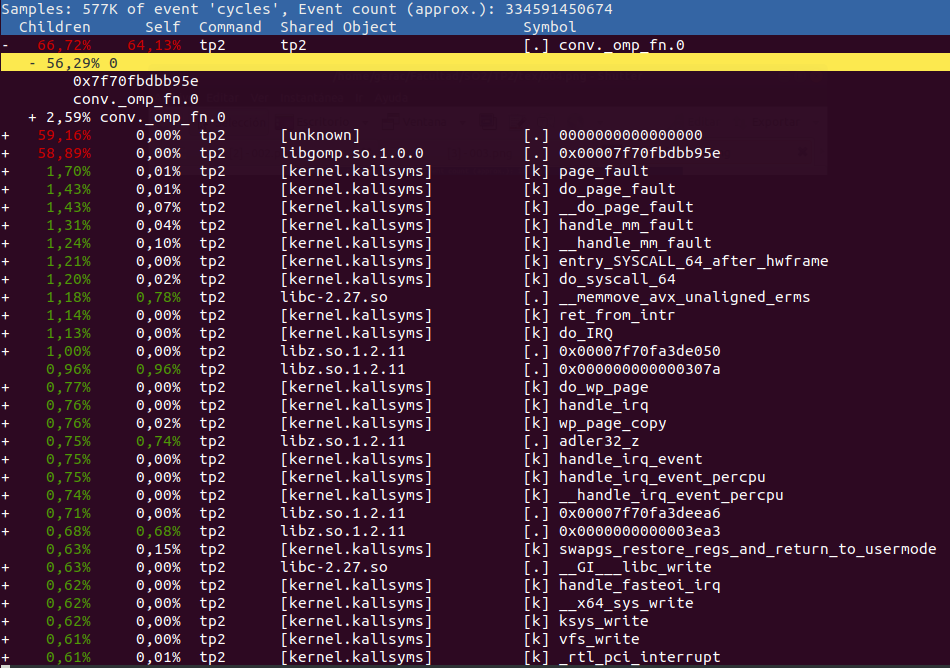
\includegraphics[width=0.9\textwidth]{005.png}
  	\caption{Llamada gráfica.}
  	\label{fig:grafcall}
  	\end{center}
\end{figure}


\subsection{\texttt{cachegrind}}
Otra herramienta de creación de perfiles es \texttt{Cachegrind}.
La traza incluye el número de accesos a la memoria de instrucciones/datos y errores de caché de primer/segundo nivel, y lo relaciona con las líneas de origen y las funciones del programa de ejecución. 

\texttt{Cachegrind} solo puede entregar un perfil plano. No existe una relación de llamada entre las funciones de una aplicación almacenada. Por lo tanto, los costos inclusivos, es decir, los costos de una función que incluye el costo de todas las funciones llamadas desde allí, no pueden calcularse. \texttt{Callgrind} extiende \texttt{Cachegrind} al incluir la relación de llamadas y el recuento exacto de eventos gastados mientras realiza una llamada.

\subsubsection{\texttt{Kcachegrind}}

Para la visualización es necesario el software \texttt{Kcachegrind}, permite un seguimiento muy fino de la traza de instrucciones a través de las diferentes librerías hasta llegar a las llamadas al sistema, definiendo cuanto \% de tiempo se lleva cada una. Todo esto a través del mapa de llamadas de la Fig. \ref{fig:callmap}. o de la interfaz mostrada en la Fig \ref{fig:grafcall}.

\begin{figure}[H]
	\begin{center}		
	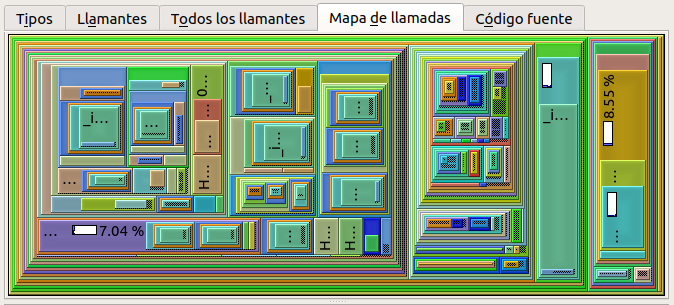
\includegraphics[width=0.7\textwidth]{007.png}
  	\caption{Mapa de llamadas.}
  	\label{fig:callmap}
  	\end{center}
\end{figure}

\begin{figure}[H]
	\begin{center}		
	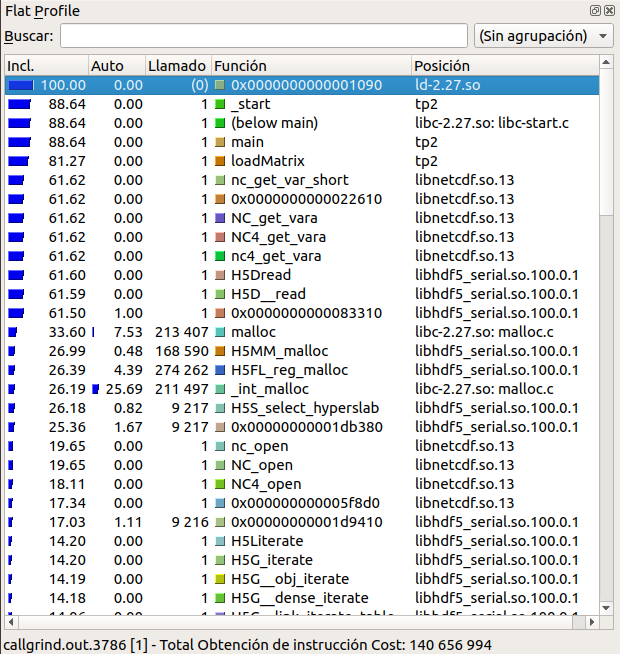
\includegraphics[width=0.7\textwidth]{006.png}
  	\caption{Perfil plano.}
  	\label{fig:grafcall}
  	\end{center}
\end{figure}

\clearpage

Cabe destacar que el software es muy interactivo y en la pestaña Gráfico de llamadas (Fig. \ref{fig:pestana}) se puede seguir a través de clicks las llamadas a funciones de todo el programa. Por último este gráfico es posible exportarlo como imagen, se adjunta al final del documento el mismo en la Fig. \ref{fig:totalgraph}.

\begin{figure}[]
	\begin{center}		
	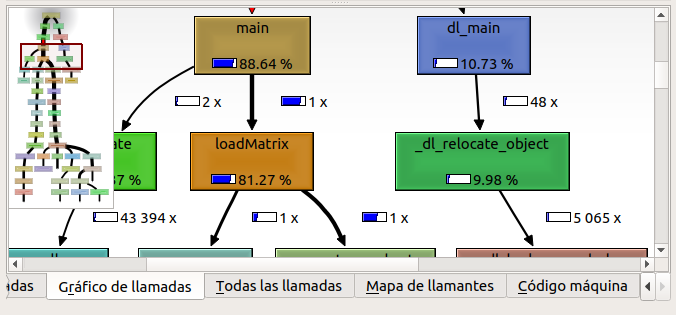
\includegraphics[width=0.9\textwidth]{008.png}
  	\caption{Pestaña de Gráfico de llamadas.}
  	\label{fig:pestana}
  	\end{center}
\end{figure}

\begin{figure}[]
	\begin{center}		
	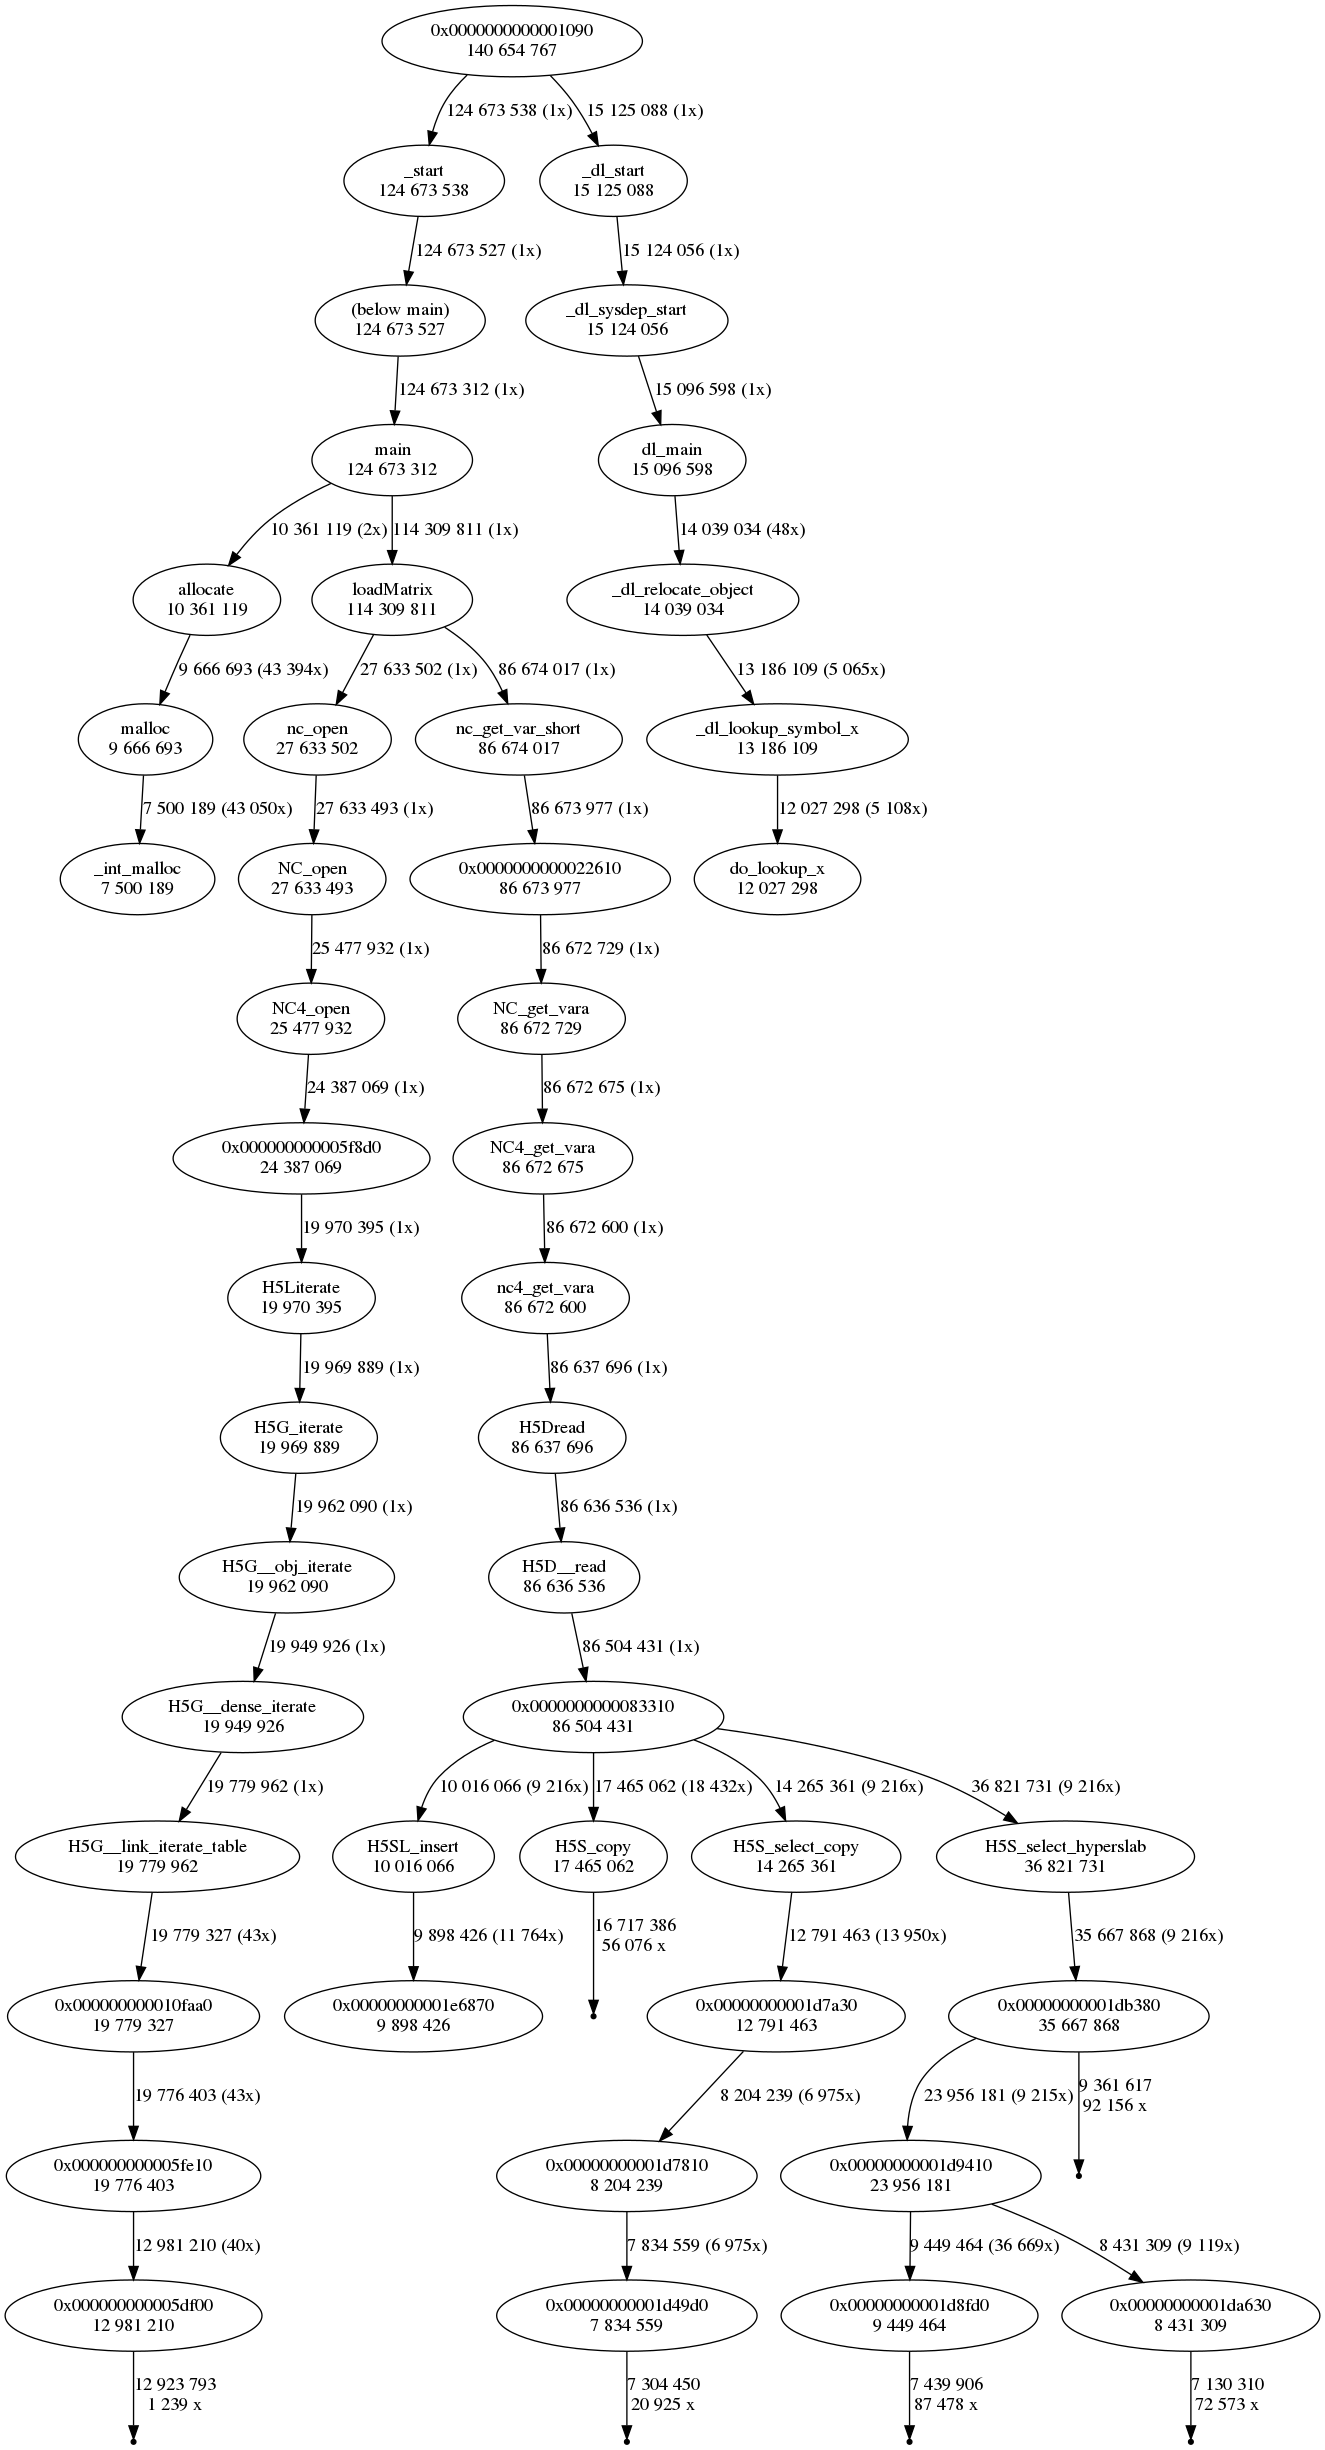
\includegraphics[width=0.9\textwidth]{output.png}
  	\caption{Gráfico de llamadas exportado.}
  	\label{fig:totalgraph}
  	\end{center}
\end{figure}

\section{Conclusión}
Se obtuvo una valiosa experiencia ya que fue un contacto directo con código capaz de manipular la cantidad de hilos utilizados para un determinado proceso. Además de ser la primera vez que se utilizaba SSH para conectarse como un host remoto.

Fue un buen vistazo al funcionamiento del procesamiento de imágenes, un campo que hoy en día está en constante expansión.

Hubo algunas dificultades con respecto a la instalación de librerías para su uso en la compilación del código pero fueron resueltas.

Con respecto al \textit{profiling} se descubrieron herramientas para esta labor y la forma en que funcionaban, siendo de gran utilidad para la mejora del código de un punto de vista plenamente objetivo. Sin embargo no fue sencillo implementar optimizaciones en base a estas porque la mayor parte del código dependía de librerías poderosas pero a su vez complejas, por tanto no se poseía mucho margen de maniobra.

\clearpage
%\bibliographystyle{ieeetr}
%\\bibliographystyle{unsrtnat}
%\\bibliography{mybib}

\end{document}
